\documentclass{article}
\usepackage{graphicx}
\usepackage{natbib}
\usepackage{subfig}

\title{Phenomenological Robotics}
\author{Bruno Nery\\
        \texttt{bnery@isr.ist.utl.pt}}

\begin{document}

\maketitle

In the world of Good Old Fashioned Artificial Intelligence (GOFAI), scientists
attempted to fabricate intelligence by doing inference on symbolic
representations of the world. 

% 1.A. "Failure" of the computational hypothesis on everyday coping (being in
% the world is more basic than thinking).
% (Source: \cite{dreyfus07}.)

Dreyfus~\cite{dreyfus07} points out that the pioneers in GOFAI learned, directly
or indirectly, from the philosophers. Hobbes' claim that reasoning was
calculating and Descartes' mental representations, among others, are cited as
examples. At the same time, he states that the critical insights formulated by
existentialist philosophers, such as Heidegger and Merleau-Ponty, were a sign
that their enterprise was comdemned to failure. He affirms that

\begin{quotation}
  Heidegger's important insight is not that, when we solve problems, we
  sometimes make use of representational equipment outside our bodies, but that
  \emph{being-in-the-world} is more basic than \emph{thinking} and solving
  problems; that it is not representational at all.
\end{quotation}

% 1.?. On Brooks attempt. On Dreyfus believe on the failure of GOFAI and Brooks.

In Brooks' \cite{brooks91} approach, this is done by making agents respond to
fixed isolable features of the environment. Dreyfus \cite{dreyfus07} believes
that the basis of human intelligence, coping with everyday life, cannot be
achieved by any of the approaches described above. Instead, the fact that

\begin{quotation}
  \dots embodied beings like us take as input energy from the physical universe
  and respond in such a way as to open them to a world organized in terms of
  their needs, interests, and bodily capacities, without their minds needing to
  impose meaning on a meaningless given \dots nor their brains converting
  stimulus input into reflex responses \dots
\end{quotation}

% 1.E. Robots have different bodies, different perceptions and different needs
%      from ours.
% (Source: Thesis journal, pages 006 to 015, 14/12/2010).

Each robot has a different body, consisting of a set of sensors and actuators. 
For this reason, a robot experiences the world in a very specific way. Its body
defines not only what it can do, but also the way in which it sees the world.
Take the HERB~\cite{srinivasa2009herb}, the iCub~\cite{metta2010icub}, and the
Pioneer P3-DX robots, for example, depicted in
Figure~\ref{fig:herb_icub_pioneer}.

\begin{figure}[h]
  \centering
  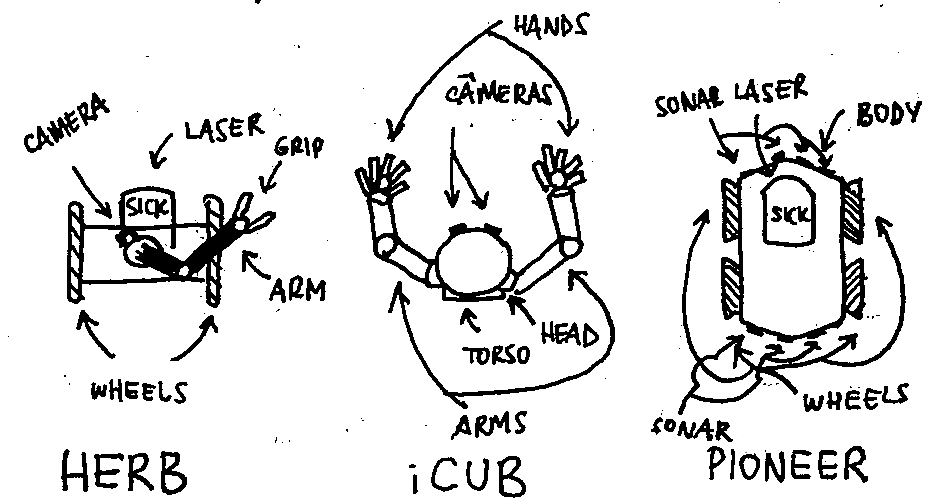
\includegraphics{figures/herb_icub_pioneer.png}
  \caption{HERB, iCub, and Pioneer P3-DX robots}
  \label{fig:herb_icub_pioneer}
\end{figure}

The HERB sees the world in \emph{forward mode} through its laser range finder
and its camera, coupled with its body movement. The iCub, in its
\emph{paraplegical} version, can only see the world in a left-to-right (and
right-to-left) manner through its cameras and head/torso movement. It can also
grasp nearby objects in order to examine them better. Finally, the Pioneer P3-DX
experiences the world in two different directions at the same time through its
sonars and its wheels movement. 

% 2. Relation between phenomenology and alternative psychology theories.

\section{Phenomenology and psychology theories}

% 2.B. Merleau-Ponty skills (refined situations) vs. Eleanor Gibson.
% (Source: Thesis journal, pages 140 to 149, 29/03/2011).
% (Source: \cite{gibson2000}.)

Dreyfus~\cite{dreyfus2002} shows that learning and skillful action, deemed as
basic forms of intelligent behavior, can be explained without recurring to
mental representations. To accomplish this, he explains the two central concepts
in Merleau-Ponty's \emph{Phenomenology of Perception}:

\begin{itemize}
\item \textbf{intentional arc:} is the strong connection between an agent and
its environment. In that sense, the skills learned by an agent are not kept as
representations in the mind, but as dispositions to respond to solicitations of
situations in the environment;
\item \textbf{maximal grip:} is the tendency of an agent to respond to these
solicitations in a way that brings the situation status closer to what it
considers optimal.
\end{itemize}

Gibson~\cite{gibson2000} propose that the process of learning is one of
discrimination rather than association, that is, through the refinement of the
sensorimotor knowledge acquired through the selection of patterns in our
interaction with the world. According to her, this selection process happens
based on two criteria:

% (\cite{gibson2000}, pages 154-156).

\begin{itemize}
\item \textbf{affordance fit:} what increases the fit between the organism and
its environment, according to its capacities and goals;
\item \textbf{economy:} what reduces the need for action and perceptual
information to accomplish a given task. -- optimization
\end{itemize}

These criteria can be seen as directly related to Merleau-Ponty's
\emph{intentional arc} and \emph{maximal grip}, respectively.

% 4. The IKEA scenario.
% (Source: Thesis journal, pages 130 to 139, 17/03/2011).

\section{The IKEA scenario}

\begin{quotation}
  A hammer is for hammering.
\end{quotation}

If you have a nail nearby, that might be the case. If you are assembling IKEA
furniture outdoors, however, a hammer might as well be ``for paper weighting''.
In the same sense, a ladder is only ``for climbing'' when you have the need to
reach a high place. Most of the times, a ladder will be
``for being in the way''.

Also, screwdrivers are, supposedly, ``for driving screws''. But what happens
when you a have a flat screwdriver and need to drive a Phillips-head screw
(Figure~\ref{fig:ikea_flat_phillips})? It is harder to drive it, but have you
ever tried driving a flat head screw with a Phillips screwdriver
(Figure~\ref{fig:ikea_phillips_flat})? It won't work, and you'll start asking
yourself what is wrong, and what you can do to fix it.

\begin{figure}[h]
  \centering
  \subfloat[][Flat screwdriver vs. Phillips-head screw] {
    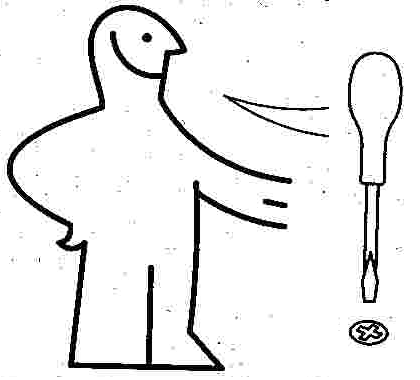
\includegraphics{figures/ikea_flat_phillips.png}
    \label{fig:ikea_flat_phillips}
  }
  \qquad
  \subfloat[][Phillips screwdriver vs. Flat head screw] {
    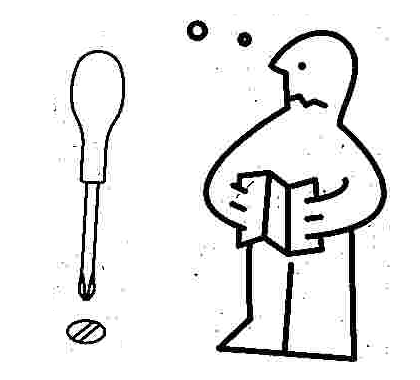
\includegraphics{figures/ikea_phillips_flat.png}
    \label{fig:ikea_phillips_flat}
  }
  \caption{The IKEA scenario}
\end{figure}

You will be having a breakdown, as described by Heidegger~\cite{dreyfus07}, and
the screwdriver will cease to be \emph{ready-to-hand} and become
\emph{present-at-hand} until you can figure out the problem. But how do we equip
a robot with the same capabilities so that it can function in a human world?

% Not present in the outline: learning process in infancy. This might not be the
% best place for this part, but it definitely goes together with the
% cornerstones of the framework below.
% (Source: Thesis journal, pages 140 to 149, 28/03/2011).
% (Source: \cite{gibson2000}, pages 134 to 149, chapter 8).

Gibson~\cite{gibson2000} affirms that perceptual learning predates birth. She
describes a number of cases, going from early perceptual learning to elaborate
sequences of action in older infants. In these cases, the infant learns:

\begin{itemize}
\item about oneself;
\item to control an event;
\item to perceive an unitary object;
\item what happens next in an observed event;
\item to participate in a communicative event;
\item to differentiate multimodally specified events;
\item distinctive features of things;
\item to use an object or an act as means;
\item about causal relations in observed events.
\end{itemize}

% Not present in the outline: cornerstones of the framework. This might not be
% the best place for this part.
% (Source: Thesis journal, pages 100 to 109, 03/03/2011).

Before a robot is able to handle a breakdown, it needs to be able to function in
the world seamlessly, fullfiling its needs by executing one action after the
other, using what is available to it in a given moment. To be able to do that,
the following set of basic capabilities might be a good place to start:

\begin{itemize}
\item \textbf{body knowledge:} know its own body, be able to detect its current
state and how it changes according to its movements;
\item \textbf{skill acquisition:} know how discover and/or learn a set of
abilities that allow it to interact with the world;
\item \textbf{object detection:} know how to single out objects and detect
properties that allow it to use them in a particular manner.
\end{itemize}

\bibliographystyle{plain}
\bibliography{prsurvey}

\end{document}
